\section{Introduction and Problem Formulation}
\label{sec:intro}

Magnetic Resonance Imaging (MRI) is a cornerstone of non-invasive medical diagnostics, yet its inherently slow acquisition time remains a critical bottleneck. Accelerating MRI typically involves undersampling the $k$-space and solving a highly ill-posed inverse problem \citep{chung2022score}. While deep generative models have achieved remarkable success in MRI reconstruction, the vast majority of these approaches operate strictly on magnitude images in the spatial domain, entirely discarding the complex phase information.

% ----------------------------------------
\begin{figure}[t]
    \centering
    \begin{subfigure}[b]{0.42\textwidth}
        \centering
        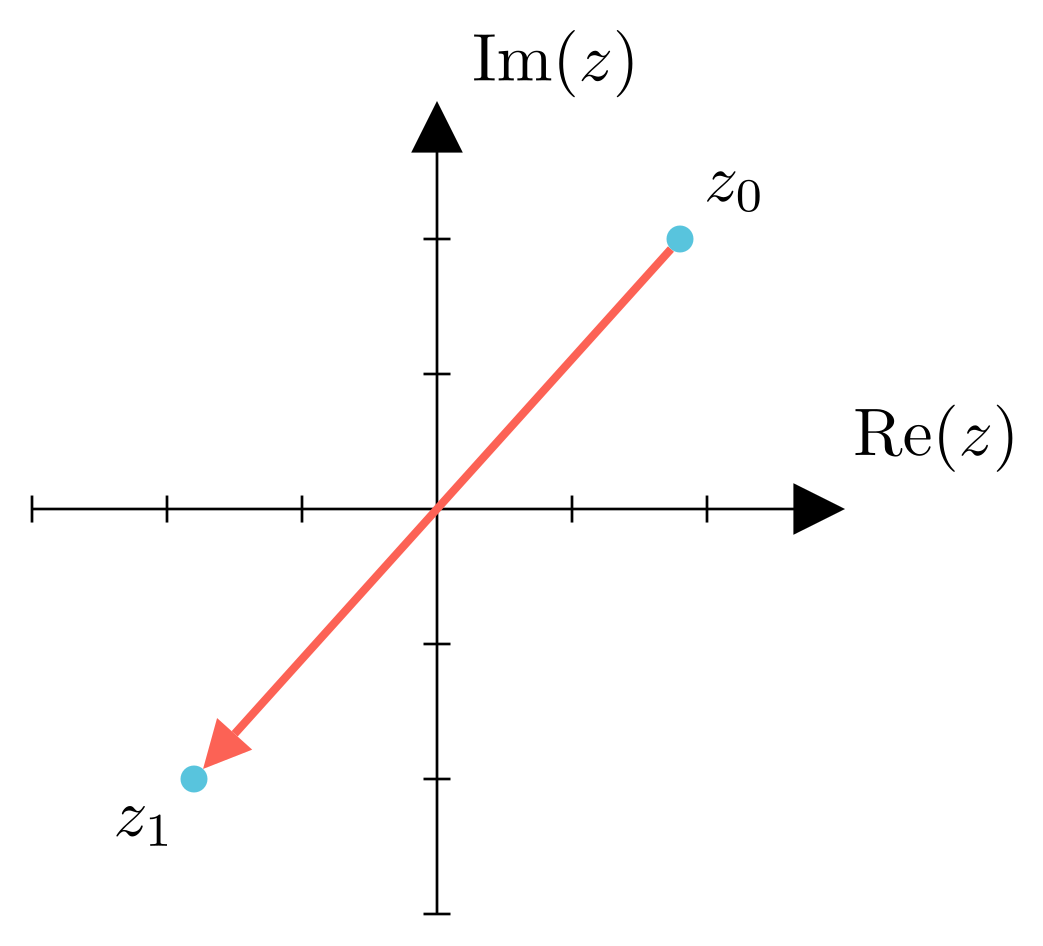
\includegraphics[height=3.2cm, keepaspectratio]{figures/EuclideanFlow_cropped.png}
        \caption{Standard Euclidean Flow ($\mathbb{R}^2$)}
        \label{fig:flow_euclidean}
    \end{subfigure}
    \hfill
    \begin{subfigure}[b]{0.42\textwidth}
        \centering
        
\includegraphics[height=3.2cm, keepaspectratio]{figures/CylindricalFlow_cropped.png}
        \caption{Cylindrical Flow Matching (Ours)}
        \label{fig:flow_cylindrical}
    \end{subfigure}
    \caption{\textbf{Topological mismatch in complex-valued generation.} \textbf{(a)} Shows the complex plane $(\mathrm{Re}(z), \mathrm{Im}(z))$, where standard models treat complex signals as flat Euclidean vectors. Linear interpolation between states $z_0$ and $z_1$ forces paths through the origin, causing destructive phase interference ($|z_{1/2}| \ll \frac{1}{2}(|z_0| + |z_1|)$) and non-physical signal cancellation. \textbf{(b)} Cylindrical Flow Matching ($S^1 \times \mathbb{R}^+$), where the probability path naturally wraps around the periodic boundary on $S^1$, preserving signal magnitude.}
    \label{fig:teaser_flow}
    \vspace{-2mm}
\end{figure}
% ---------------------------------------- 

This magnitude-only paradigm creates a significant research gap. Recently, emerging diagnostic systems have begun to explore the immense potential of operating directly on complex-valued data in the frequency domain, demonstrating that complex neural networks can better preserve signal fidelity and crucial physiological information in raw MRI processing \citep{rempe2026kvit, dou2025mri}. However, the lack of realistic, fully complex synthetic $k$-space data severely hinders the broad development and validation of such architectures. Although recent diffusion-based approaches have begun to explore complex-valued data generation to address this scarcity \citep{rempe2025phasegen}, robust and geometrically accurate generative baselines are still lacking. Furthermore, while state-of-the-art counterfactual generators provide valuable interpretability in the spatial domain \citep{bedel2024dreamr, min2025instructx2x}, their lack of complex-domain constraints makes them prone to hallucinating non-physical pixel values. Upon Inverse Fast Fourier Transform (IFFT), these spatial modifications violate topological validity and leak into measured $k$-space subspaces, creating high-frequency artifacts.

To safely develop frequency-domain Explainable AI (XAI) and reliable generative models, frameworks must synthesize fully complex data while respecting physical laws. Yet, current approaches suffer from a fundamental topological mismatch. They naively treat the complex signal as a flat, two-channel tensor (concatenating real and imaginary parts) embedded in a Euclidean space $\mathbb{C} \cong \mathbb{R}^2$ \citep{chung2022score}. This assumption is fundamentally flawed as it completely ignores the intrinsic circular topology ($S^1$) of the signal's phase. Standard Euclidean interpolation suffers from destructive interference due to the triangle inequality:
\begin{equation}
    |z(t)| = |(1-t)z_0 + t z_1| \le (1-t)|z_0| + t|z_1|
\end{equation}
with strict inequality whenever phases differ ($\theta_0 \ne \theta_1$). Measured empirically on the SKM-TEA dataset at $t = 0.5$, the mean amplitude ratio $\frac{|z_{1/2}|}{\frac{1}{2}(|z_0| + |z_1|)}$ drops to $0.8417$, demonstrating an average $\sim$16\% non-physical signal power loss in real MRI data. Furthermore, such flat interpolation fails to capture the continuous wrapping at the boundaries ($-\pi$ and $\pi$). In the context of safety-critical medical downstream tasks, such geometric violations are disqualifying. 

To bridge the gap between generative modeling and the structured nature of physical signals, we propose \textbf{Cylindrical Flow Matching}, a geometry-aware generative framework designed specifically for complex-valued medical image synthesis. Building on flow matching \citep{lipman2023flow} and its manifold extension \citep{chen2024flow}, we explicitly model the amplitude on $\mathbb{R}^+$ and the phase on a circular manifold $S^1$, naturally respecting the periodic topology of the MRI phase signal. 

Crucially, despite operating on a non-Euclidean cylindrical manifold, our approach preserves mathematical elegance and computational efficiency. The probability paths on $S^1$ are constructed along geodesics using logarithmic and exponential maps, resolving the transport to the shortest angular distance and effortlessly crossing periodic boundaries without the need for heuristic penalty terms \citep{chen2024flow}. Using comprehensive raw $k$-space datasets such as SKM-TEA, we demonstrate that substituting the standard Euclidean manifold with a cylindrical one natively resolves phase discontinuities, ensuring topological validity and physical signal plausibility, and providing a reliable source of synthetic complex-valued data for downstream clinical applications.
